\section{The Groupoid of Finite Types}
\label{sec:ufin}

% First - recap the previous section
% Second - say what was wrong

Using categorical language, the setting for the semantics in the previous section is the category of finite sets and
functions $\SetFin$. However, as $\PiLang$ only refers to bijective functions, a more precise setting is the groupoid
$\BFin = \term{core}(\SetFin)$ of finite sets and bijections. $\SetFin$ has finite coproducts $(\emptyt, \sqcup)$ and
finite products $(\unit, \times)$ and in $\BFin$ these restrict to additive and multiplicative symmetric monoidal
structures, respectively, making $\BFin$ a symmetric rig groupoid -- the \emph{vertical categorification} of the
commutative rig of natural numbers $\Nat$.

The semantics interprets $\PiLang$-types as objects in $\BFin$, 1-combinators as isomorphisms, and for every pair of 1-combinators
related by a 2-combinator, their interpretations in~$\BFin$ are equal.  The groupoid $\BFin$ is strict, since the
collection of isomorphisms is a set, that is, a discrete category. There is no explicit witness for the equality of two
isomorphisms, since we can decide by evaluating two bijections whether they are equal. To be able to establish
completeness for $\PiLang$, we want a witness for this equality, so that we can quote back to the syntax and produce a
2-combinator witnessing the equality of the corresponding 1-combinators.

% The denotational semantics for $\PiLang$ in the previous section uses the symmetric rig groupoid structure of $\BFin$,
% whose objects are finite sets, whose morphisms as bijections between finite sets, and whose symmetric monoidal
% structures are induced by the operations $\sqcup$ and $\times$. The

% two equal permutations are extensionally identified, without an explicit witness for the equality. In order to
% establish completeness, we want to quote back from the semantics to the syntax. Specifically, given a morphism in
% $\BFin$, we want to produce a 1-combinator in $\PiLang$, and given two extensionally equal morphisms in $\BFin$, we
% want to produce a 2-combinator witnessing the equality of the quoted 1-combinators.

% Third - say how are we fixing it

We observe that the implicit equalities between the isomorphisms are pointwise equalities of functions, that is,
homotopies. We therefore \emph{weaken} the groupoid $\BFin$, exposing these homotopies, by using higher invertible cells
and work in HoTT (Univalent Foundations) as it provides a proof-relevant, constructive metatheory to get a handle
on these equalities and provides a rich internal language for describing weak groupoids, using the ``types are weak
$\infty$-groupoids'' correspondence.

% To get a handle on these equalities, we will work in a proof-relevant metatheory, that is, HoTT, and then we will
% be able to write functions out of them back into the syntax.

% HoTT provides a rich internal language for describing weak groupoids.

% The idea is that we move from (discrete) sets to proof-relevant $\hSet$s, where the type of equalities between two
% points in a set is a proposition, that is, a prop-enriched groupoid.

% Our first step is therefore to expose the implicit equalities by \emph{weakening} the groupoid $\BFin$, i.e., by
% replacing the equational axioms of the category by higher invertible cells. In a weak category, the identity and
% associativity equational conditions are replaced by higher cells for the left and right units of composition and for
% associativity; these higher cells come with their own coherence data as well, such as vertical composition, and
% horizontal composition, or whiskering as detailed in appendix~\ref{app:twocat}.

% Fourth - explain the tool we use for fixing it
Every type in HoTT is a weak $\infty$-groupoid whose points are the terms of the type, and the (iterated) identity type
gives the (higher) morphisms. The groupoid we are interested in has types as points, type equivalences for 1-cells, and
higher homotopies for higher cells. (See App.~\ref{app:grpdexample} for an example on a 3-element set.) This is the
groupoid structure for the universe type $\UU$, since the identity type on types can be characterised as type
equivalences (by \emph{univalence}). But, we only want to carve out a \emph{subuniverse} of \emph{finite types}, still
satisfying univalence, to get the groupoid structure. In this section, we formally define \emph{univalent subuniverses},
and proceed to construct the particular instance for finite types, $\UFin$ (\Cref{def:ufin}).

% The way to describe such groupoid in HoTT is to construct a type which has the types themselves as points, i.e. a
% universe. Then, equivalences between those types can be characterized using elements of the equality type. For this to
% work, the universe in question has be a \emph{univalent subuniverse}.

% In HoTT, every type carries a groupoid structure, with terms for points, and the (iterated) identity type for (higher)
% morphisms. We're interested in the groupoid structure of the universe, which has types for points, equivalences for
% identities between them (by univalence), and higher homotopies for higher identifications. We want a similar
% universe, whose only points are the finite types, that is, a subuniverse, and, equalities between them should
% correspond to equivalences of finite types -- the subuniverse should be univalent. To construct a univalent
% subuniverse starting from a univalent universe, we will introduce the concept of univalent fibrations.

% However, although weakening the groupoid exposes some implicit equalities, it does not, by itself, give us a handle to
% characterize such equalities. One elegant way to acquire such an ability is to ensure that the groupoid is
% ``univalent,'' as this provides a way to characterize the semantic equivalences using the elements of the identity
% type, i.e., using objects whose equality is equipped with an induction principle. We will therefore work within a HoTT
% metatheory which provides an ambient univalent universe of types and introduce the novel idea of a \emph{univalent
% subuniverse} to carve out $\UFin$: a weakened, univalent, version of the groupoid $\BFin$ which is then extended with
% the appropriate commutative rig structure. The main technical result of this section that is exploited in the next
% section is that, for each finite type $T$, we have transferred the structure of the space of equivalences $T \eqv T$
% to the structure of paths in $\UFin$. Since the space equivalences forms the automorphism group of $T$, we can now use
% the tools of computational group theory together with the induction principle of paths and term rewriting theory to
% describe the paths in $\UFin$.

% HoTT provides a rich internal language for working with weak higher groupoids, using the ``types are weak
% $\infty$-groupoids'' correspondence. In this section, we show that the weakened version of the groupoid $\BFin$ can be
% written in HoTT as a type $\UFin$, which is a 1-groupoid that has points for 0-cells, 1-paths for 1-cells, 2-paths for
% 2-cells with at most one 2-cell between compatible 1-cells.

%% In this section, we develop the tools necessary to construct $\UFin$, starting with a quick review of HoTT. % Using
%the identity type for morphisms, a 1-groupoid in HoTT

% IS THAT FOOTNOTE NECESSARY ??? We should avoid using footnotes as much as possible.\footnote{This is a locally-strict
%   $(2,0)$-category, since every cell above 0 is invertible, and the hom-categories are posets, that is, truth-value
%   enriched.}

\begin{toappendix}
  \label{app:grpdexample}
  We give an example of the groupoid structure on a 3-element set.

  \[
    \begin{tikzcd}
      \Fin[3]
      \arrow[""{name=0, anchor=center, inner sep=0}, "{f_{3}}", no head, loop, distance=4em, in=115, out=65]
      \arrow[""{name=0, anchor=center, inner sep=0}, "{f_{2}}", no head, loop, distance=8em, in=125, out=55]
      \arrow[""{name=1, anchor=center, inner sep=0}, "{f_{1}}"', no head, loop, distance=12em, in=135, out=45]
      \arrow["", "{h}", shorten <=3pt, shorten >=3pt, Rightarrow, no head, from=0, to=1]
    \end{tikzcd}
  \]

  \noindent We have $\Fin[3] = \Set{0,1,2} \eqv \unit \sqcup (\unit \sqcup \unit)$ which fixes a particular enumeration of the
  elements. Suppose we have a set $X = (\unit \sqcup \unit) \sqcup \unit$, it has the same cardinality as $\Fin[3]$, so it
  is represented by the same 0-cell. But, $X$ can be made equivalent to $\Fin[3]$ in many different ways since there are
  many bijections between them. One bijection is
  $\Set{\inl(\inl(\ttt)) \mapsto 0, \inl(\inr(\ttt)) \mapsto 1, \inr(\ttt) \mapsto 2}$ which can be written in two
  different ways by composing more primitive operations, $f_{1} = \assocrp$, or
  $f_{2} = \swapp \compc \assoclp \compc \swapp$. Another bijection is
  $\Set{\inl(\inl(\ttt)) \mapsto 1, \inl(\inr(\ttt)) \mapsto 2, \inr(\ttt) \mapsto 0}$ which is given by $f_{3} = \ldots$.
  Since $f_{1}$ and $f_{2}$ produce the same enumeration of the elements of $X$, they are identified by a homotopy $h$
  which is encoded in the 2-cell between them.

  At level 0, all we know is that if $X : \UFin[3]$, then X is merely equal to $\Fin[3]$, that is
  $\Trunc[-1]{X \id \Fin[3]}$, and we don't have access to the bijection. At level 1, if we know that both $X$ and $Y$ are
  \emph{equal} in $\UFin[3]$, then we can extract an equivalence between them, that is, $(X \id Y) \to (X \eqv Y)$.
  $\UFin[3]$ being a univalent subuniverse asserts that there are as many elements (upto higher homotopy) in $X \id Y$ as
  there are $X \eqv Y$.
\end{toappendix}

% \begin{toappendix}

%   \subsection{To Put Somewhere or Delete}

%   This approach is sufficient to prove the semantics forms a 1-category but ignores the rich structure at the next
%   level~\cite{carette2016}.
%   As explained in the previous section, a $\Pi$-type $A$ has $\sizet{A}$-elements and for all combinators $c : A \iso B$
%   we have that $\sizet{A} = \sizet{B}$. Hence, the denotation $\denot{A}$ of a type $A$ with $n$-elements can be the finite
%   set $\Fin[n] = \{ 0, 1, \cdots, n-1\}$; the denotation of a value $v : A$ such that $\sizet{A}=n$ will be an index in
%   the range $[0,n-1]$, and the denotation $\denot{c}$ of a combinator $c : A \iso B$ such that
%   $\sizet{A} = \sizet{B} = n$ will be a function from $\Fin[n]$ to $\Fin[n]$ that permutes the elements. Thus, all types
%   with 3 elements will denote $\Fin[3]$ and combinators between them will denote permutations on $\Fin[3]$, e.g.:
%   \[\begin{array}{rcl}
%       \denot{\onet + (\onet + \onet)}                                         & = & \{ 0,1,2 \} \\
%       \denot{(\onet + \onet) + \onet}                                         & = & \{ 0,1,2 \} \\
%       \\
%       \denot{\assoclp : \onet + (\onet + \onet) \iso (\onet + \onet) + \onet} & = & (0~1~2)     \\
%       \denot{\swapp : \onet + (\onet + \onet) \iso (\onet + \onet) + \onet}   & = & (2~0~1)
%     \end{array}\]
%   where we have used the one-line notation for permutations with $(a~b~c)$ representing the
%   permutation that maps 0 to $a$, 1 to $b$, and 2 to $c$. To make the denotation of values precise, we compute a canonical
%   enumeration of the elements of each type:
%   \[\begin{array}{rcl}
%       \mathit{enum}(\zerot)     & = & [~]                                                                                                          \\
%       \mathit{enum}(\onet)      & = & [ ~\Acon{tt}~ ]                                                                                              \\
%       \mathit{enum}(A + B)      & = & \mathit{map}~\Acon{inj₁}~\mathit{enum}(A) ~\textsf{+\!+}~ \mathit{map}~\Acon{inj₂}~\mathit{enum}(B)          \\
%       \mathit{enum}(A \times B) & = & \mathit{concat}~(\mathit{map}~(\lambda v.\mathit{map}~(\lambda w. (v,w))~\mathit{enum}(B))~\mathit{enum}(A))
%     \end{array}\]
%   \noindent The specification uses a Haskell-like notation for sequences with $\mathit{map}$ as the operation that applies
%   a function to each element of a sequence, \textsf{+\!+} as the binary append operation, and $\mathit{concat}$ the
%   operation that appends all the subsequences in a sequence.

%   Using the definition, we have:
%   \[\begin{array}{rcl}
%       \mathit{enum}(\onet + (\onet + \onet)) & = & [ \inlv{\Acon{tt}},~\inrv{(\inlv{\Acon{tt}})},~\inrv{(\inrv{\Acon{tt}})} ] \\
%       \mathit{enum}((\onet + \onet) + \onet) & = & [ \inlv{(\inlv{\Acon{tt}})},~\inlv{(\inrv{\Acon{tt}})},~\inrv{\Acon{tt}} ]
%     \end{array}\]
%   Thus, as shown in the diagrams below, $\assoclp~(\inlv{\Acon{tt}})$ applies the permutation $(0~1~2)$ to the index of
%   $\inlv{\Acon{tt}}$ which is 0 and produces index 0 in the $(\onet + \onet) + \onet$ type corresponding to value
%   $\inlv{(\inlv{\Acon{tt}})}$. Similarly, $\swapp~(\inlv{\Acon{tt}})$ applies the permutation $(2~0~1)$ to the index of
%   $\inlv{\Acon{tt}}$ which is 0 and produces index 2 in the $(\onet + \onet) + \onet)$ type corresponding to value
%   $\inrv{\Acon{tt}}$.

%   \begin{center}
%     \begin{tikzpicture}[scale=0.8,every node/.style={scale=0.8}]
\node at (-3,1.3) {$\mathit{enum}$};
\node at (-1,1.3) {$\assoclp$};
\node at (0.7,1.3) {$\mathit{enum}$};
	\begin{pgfonlayer}{nodelayer}
		\node (4) at (-4, 1) {$\inlv{\Acon{tt}}$};
		\node (0) at (-4, 0) {$\inrv{(\inlv{\Acon{tt}})}$};
		\node (5) at (-4, -1) {$\inrv{(\inrv{\Acon{tt}})}$};

		\node (6) at (-2, 1) {0};
		\node (1) at (-2, 0) {1};
		\node (7) at (-2, -1) {2};

		\node (8) at (0, 1) {0};
		\node (2) at (0, 0) {1};
		\node (9) at (0, -1) {2};

		\node (10) at (2, 1) {$\inlv{(\inlv{\Acon{tt}})}$};
		\node (11) at (2, 0) {$\inlv{(\inrv{\Acon{tt}})}$};
		\node (12) at (2, -1) {$\inrv{\Acon{tt}}$};
	\end{pgfonlayer}
	\begin{pgfonlayer}{edgelayer}
		\draw[->] (4) to (6);
		\draw[->] (0) to (1);
		\draw[->] (5) to (7);
		\draw (6) to (8);
		\draw (1) to (2);
		\draw (7) to (9);
		\draw[<-] (8) to (10);
		\draw[<-] (2) to (11);
		\draw[<-] (9) to (12);
	\end{pgfonlayer}
\end{tikzpicture}

%     \qquad
%     \begin{tikzpicture}[scale=0.8,every node/.style={scale=0.8}]
\node at (-3,1.3) {$\mathit{enum}$};
\node at (-1,1.3) {$\swapp$};
\node at (0.7,1.3) {$\mathit{enum}$};
	\begin{pgfonlayer}{nodelayer}
		\node (4) at (-4, 1) {$\inlv{\Acon{tt}}$};
		\node (0) at (-4, 0) {$\inrv{(\inlv{\Acon{tt}})}$};
		\node (5) at (-4, -1) {$\inrv{(\inrv{\Acon{tt}})}$};

		\node (6) at (-2, 1) {0};
		\node (1) at (-2, 0) {1};
		\node (7) at (-2, -1) {2};

		\node (8) at (0, 1) {0};
		\node (2) at (0, 0) {1};
		\node (9) at (0, -1) {2};

		\node (10) at (2, 1) {$\inlv{(\inlv{\Acon{tt}})}$};
		\node (11) at (2, 0) {$\inlv{(\inrv{\Acon{tt}})}$};
		\node (12) at (2, -1) {$\inrv{\Acon{tt}}$};
	\end{pgfonlayer}
	\begin{pgfonlayer}{edgelayer}
		\draw[->] (4) to (6);
		\draw[->] (0) to (1);
		\draw[->] (5) to (7);
		\draw (6) to (9);
		\draw (1) to (8);
		\draw (7) to (2);
		\draw[<-] (8) to (10);
		\draw[<-] (2) to (11);
		\draw[<-] (9) to (12);
	\end{pgfonlayer}
\end{tikzpicture}

%   \end{center}


%   We choose a canonical set of size $n$, called $\mathsf{Fin}~n$, whose elements are natural numbers less than $n$. To
%   compute the denotation of a type $A$, we first calculate its size $n = \sizet{A}$. We then construct the canonical set
%   $\mathsf{Fin}~n$ and provide the (trivial) evidence that this set is identical to $(\mathsf{Fin}~n)$:

%   \[\begin{array}{rcll}
%       \sem{A} & = & (\mathsf{Fin}~n, [ n , \mathsf{refl} ]) & \mbox{where}~\sizet{A} = n
%     \end{array}\]

%   \noindent The denotation $\sem{c}$ of a combinator $c : A \isoone B$ is a path between $\sem{A}$ and $\sem{B}$. If the
%   size of $A$ is $m$ and the size of $B$ is $n$, the desired path is between $(\mathsf{Fin}~m, [ m , \mathsf{refl} ])$ and
%   $(\mathsf{Fin}~n, [ n , \mathsf{refl} ])$. This path is directly constructed using $\mathit{ap}$ and the fact that $m=n$
%   since combinators are always between types of the same size.

%   \noindent Finally, given two combinators $p , q : A \isoone B$ and a 2-combinator $\alpha : p \isotwo q$, the denotation
%   $\sem{\alpha}$ of $\alpha$ is a path between $\sem{p}$ and $\sem{q}$.

%   \note{We use the rig structure of $\UFin$ in~\Cref{subsec:rig} to interpret $\PiLang$.}


%   We need a formal definition of normal form (canonical form)

%   Recalling that the $\lambda$-calculus arises as the internal language of Cartesian Closed Categories
%   (Elliott~\cite{Elliott-2017} gives a particularly readable account of this), we can think of $\Pi$ in similar terms, but
%   for symmetric Rig Groupoids instead. For example, we can ask what does the equivalence above represent? It is actually a
%   ``linear'' representation of a 2-categorial commutative diagram! In fact, it is a painfully verbose version thereof, as
%   it includes many \emph{refocusing} steps because our language does not build associativity into its syntax. Categorical
%   diagrams usually do.  Thus if we rewrite the example in diagrammatic form, eliding all uses of associativity, but
%   keeping explicit uses of identity transformations, we get that \AgdaFunction{swap{-}fl2⇔swap{-}fl1} represents

%   \vspace*{3mm}
%   \begin{tikzcd}[column sep=normal, row sep=normal]
%     && (a+c)+b \arrow [r, "\swapp \oplus\idd", ""{name=U, below}] & (c+a)+b \arrow [dr, "\assocrp"] && \\
%     & a+(c+b) \arrow [ur, "\assoclp"] & & & c+(a+b) \arrow [dr, "\idd\oplus\swapp"] &  \\
%     a+(b+c) \arrow [ur, "\idd\oplus\swapp"] \arrow [r, "\assoclp"]
%     \arrow [dr, "\assoclp"]
%     \arrow [ddr, swap, "\assoclp"]
%     & (a+b)+c \arrow [r, "\swapp"] &
%     c+(a+b) \arrow [r, swap, "\assoclp", ""{name=D, above}]
%     & |[alias=Z]| (c+a)+b \arrow [r, "\assocrp"] &c+(a+b) \arrow [r, "\idd\oplus\swapp"] & c+(b+a) \\
%     & (a+b)+c \arrow [dr, "\swapp"] &&&& \\
%     & (a+b)+c \arrow [dr, swap, "\swapp"] & c+(a+b) \arrow [rr, swap, "\idd", ""{name=DD, above}]
%     \arrow [d, Rightarrow, "\idf\, \mathit{idl}\odot{l}"] &&
%     c+(a+b) \arrow [ruu, "\idd\oplus\swapp"] & \\
%     && c+(a+b) \arrow [rrruuu, bend right = 40, swap, "\idd\oplus\swapp"] && \\
%     \arrow[Rightarrow, from=U, to=D, "\mathit{hexagon}\oplus{r}\, \boxdot\, \idf"]
%     \arrow[Rightarrow, from=Z, to=DD, swap, "\idf\boxdot\mathit{linv}\odot{l}\,\boxdot\,\idf"]
%   \end{tikzcd}

% \end{toappendix}

%%%
\subsection{The Type Theory}~\label{subsec:type-theory}
% \subsection{Univalent Subuniverses}
% \label{sec:univalent}

% In order to define the weak groupoid we're after, we seek a mathematical structure satisfying the following properties:
% (i) it contains structures corresponding to all the finite types and nothing but the finite types, and (ii) it is robust
% enough to ensure that equivalent encodings of finite types are identified.

We use the type theory of the HoTT book~\cite{univalentfoundationsprogramHomotopyTypeTheory2013}, that is, we use
intensional Martin-L\"{o}f Type Theory, with a (univalent) universe $\UU$, and a few Higher Inductive Types (HITs) for
propositional and set truncation, and set-quotients. All arguments will hold in a Cubical Type
Theory~\cite*{cohenCubicalTypeTheory2018,angiuliComputationalSemanticsCartesianCubical2019,vezzosiCubicalAgdaDependently2019}
as well.  In App.~\ref{app:identitytypes}, App.~\ref{app:homotopytypes}, and App~\ref{app:hits}, we review the basics of
identity types, homotopy types, and HITs and refer the reader to the book for more details.

% To recap, types in HoTT have a weak groupoid structure given by the identity type, where points are given by terms of
% the type, and higher morphisms are given by the iterated identity type. Functions between types are functors between
% groupoids, and type families, or functions to the universe, are indexed families of groupoids.

\begin{toappendix}
  \subsection{Identity Types}
  \label{app:identitytypes}

  Given two terms $x:A$ and $y:A$, we write $x \id_{A} y$, or simply $x \id y$, for the identity type, which is the type
  of equalities or identifications between them. The identity type is generated by reflexivity $\refl_{x} : x \id_{A} x$,
  and the eliminator for the identity type is given by path induction or the $J$-rule (\Cref{def:path-induction}). This
  construction can be iterated, giving the identity type between two terms of an identity type, repeating ad infinitum.
  Using the iterated identity type for morphisms, each type is equipped with the structure of a weak $\infty$-groupoid,
  where each morphism satisfies groupoid laws only upto a higher one. Given an arbitrary type (or groupoid) $A$, we list
  some laws that are provable using path induction.

  \begin{definition}[Path Induction]
    \label{def:path-induction}
    Given a type family $C : \dfun{x,y:A}{(x \id_A y)} \to \UU$, and a function $c : \dfun{x:A}{C(x,x,\refl_x)}$, there is
    a function $f : \dfun{x,y:A}{\dfun{p:x \id_A y}{C(x,y,p)}}$ such that $f(x,x,\refl_x) \defeq c(x)$.
  \end{definition}

  \begin{gather*}
    \begin{aligned}
      \term{\inv{\blank}}      & : (x \id_{A} y) \to (y \id_{A} x)                   \\
      \term{\blank\comp\blank} & : (x \id_{A} y) \to (y \id_{A} z) \to (x \id_{A} z)
    \end{aligned}
    \qquad
    \begin{aligned}
      \term{assoc} & : (p : x \id_{A} y)  (q : y \id_{A} z) (r : z \id_{A} w) \\
                   & \to (p \comp q) \comp r \id p \comp (q \comp r)          \\
      \term{invr}  & : (p : x \id_{A} y) \to p \comp \inv{p} \id \refl_{x}
    \end{aligned}
  \end{gather*}

  \noindent A homotopy between functions $f \htpy g$ is given by pointwise equality between them $\dfun{x:A}{f(x) \id_{B} g(x)}$.
  The identity type for functions is equivalent to homotopies between them ${(f \id_{A \to B} g)} \eqv {(f \htpy g)}$, by
  function extensionality. An equivalence between types $A \eqv B$ is given by a pair of functions between them which
  compose to the identity, $f \comp g \htpy \idfunc_{B}$ and $g \comp f \htpy \idfunc_{A}$, and this is equivalent to the
  identity type for the universe, $(A \id_{\UU} B) \eqv (A \eqv B)$, by univalence.


  Functions between types are functors between groupoids. Given a function $f : A \to B$, there is a functorial action on
  the paths given by $\term{ap}$. Type families, that is, types indexed by terms, are simply functions from a type to the
  universe, such as $A \to \UU$. For a type family $P : A \to \UU$ and a point $x : A$, the type $P(x)$ is called the
  fiber over $x$.  The $\term{transport}$ operation, named $\term{tr}$, lifts paths in the indexing type to functions
  between fibers.
  %which is an $A$-indexed family of groupoids.

  \begin{gather*}
    \term{ap}_{f} : \dfun{x,y:A}{x \id_{A} y \to f(x) \id_{B} f(y)}
    \qquad
    \term{tr}_{P} : \dfun{x,y:A}{x \id_{A} y \to P(x) \to P(y)}
  \end{gather*}

  The type $\dsum*{x:A}{P(x)}$ is the collection of all the fibers and is called the total space of $P$. The first
  projection ${\pi_1 : \dsum*{x:A}{P(x)} \to A}$ from the total space to the base space $A$ has the structure of a
  fibration, that is, there is a lifting operation (\Cref{fig:lift}) which lifts paths in the base space to paths in the
  total space. Given a path $p : x \id_{A} y$ in the base space, and $u : P(x)$ a point in the fiber over $x$, we have:

  \[
    \term{lift}(u,p) : (x , u) \id_{\dsum{x:A}{P(x)}} (y , \transport{P}{p}{u})
  \]

  % where $\tr{p}{u}$ is shorthand for $$.

  \begin{figure}
    \begin{center}
      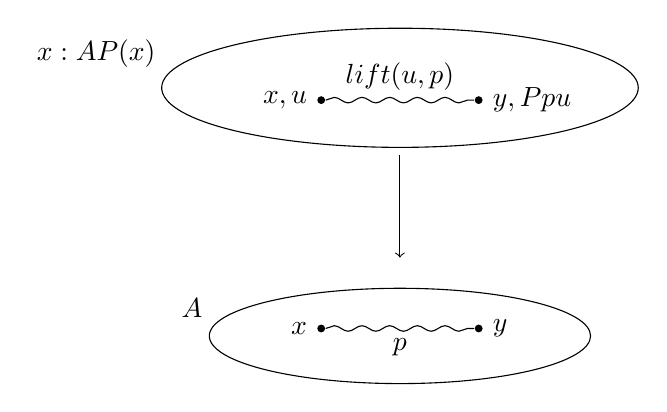
\begin{tikzpicture}[yscale=.5,xscale=2]
        \draw (0,0) arc (-90:170:8ex) node[anchor=south east] {$A$} arc (170:270:8ex);
        \draw (0,6) arc (-90:170:10ex) node[anchor=south east] {$\dsum{x:A}{P(x)}$} arc (170:270:10ex);
        \draw[->] (0,5.8) -- node[auto] {$\fst$} (0,3.2);
        \node[circle,fill,inner sep=1pt,label=left:{$x$}] (b1) at (-.5,1.4) {};
        \node[circle,fill,inner sep=1pt,label=right:{$y$}] (b2) at (.5,1.4) {};
        \draw[decorate,decoration={snake,amplitude=1}] (b1) -- node[auto,swap] {$p$} (b2);
        \node[circle,fill,inner sep=1pt,label=left:{$\pair{x,u}$}] (b1) at (-.5,7.2) {};
        \node[circle,fill,inner sep=1pt,label=right:{$\pair{y,\transport{P}{p}{u}}$}] (b2) at (.5,7.2) {};
        \draw[decorate,decoration={snake,amplitude=1}] (b1) -- node[auto] {$\term{lift}(u,p)$} (b2);
      \end{tikzpicture}
    \end{center}
    \caption{Lifting operation in $P$}
    \label{fig:lift}
  \end{figure}

\end{toappendix}

\subsection{Univalent Fibrations}

Functions between types are functors between groupoids, and type families (or functions to the universe) are indexed
families of groupoids. A type family $P : A \to \UU$ comes equipped with a functor $\pi_1 : \dsum*{x:A}{P(x)} \to \UU$
which has a lifting operation giving it the structure of a fibration. The
$\term{transport}$ operation $\transport{P}{p}{\blank}$ lifts paths in the base space to equivalences between the fibers:
% Using the groupoid structure of
% $A$, we can show that $\transport{P}{p}{\blank}$ and $\transport{P}{\inv{p}}{\blank}$ form an equivalence.
% We name
% this map $\tptEqv{P}$ which lifts paths to equivalences of fibers.
\[
  \tptEqv{P} : \dfun{x,y:A}{x \id_{A} y \to P(x) \eqv P(y)}
\]

\noindent The type families (or fibrations) we are interested in are the ones where paths in the base space completely determine
the equivalences in the fibers -- these are called univalent
fibrations~\cite*{kapulkinUnivalenceSimplicialSets2018,kapulkinSimplicialModelUnivalent2021,christensenCharacterizationUnivalentFibrations2015}.

\begin{definition}[Univalent Fibration]
  $P$ is a univalent type family (or, $\fst : {\dsum*{x:A}{P(x)}} \to A$ is a univalent fibration) if $\tptEqv{P}$ is an
  equivalence.
\end{definition}

The use of the word \emph{univalent} here is a reference to Voevodsky's \emph{univalence} principle. Indeed, univalence
characterises paths in the universe as equivalences between types, which follows from the canonical fibration
$\idfunc : \UU \to \UU$ being univalent.

\begin{toappendix}

  \subsection{Homotopy Types}
  \label{app:homotopytypes}

  A type is \emph{contractible} (-2-type) if it has a unique element, that is, there is a center of contraction and every
  other point is equal to it. A type is a \emph{proposition} (-1-type) if its equality types are contractible, that is, it
  has at most one inhabitant. Iterating this, we can define sets or 0-types (whose equality types are propositions) and
  1-groupoids or 1-types (whose equality types are sets), and similarly, higher homotopy $n$-types.

  \begin{gather*}
    \begin{aligned}
      \isContr{A} & \defeq \dsum{x:A}{\dfun{y:A}{y \id x}} \\
      \isProp{A}  & \defeq \dfun{x,y:A}{\isContr{x \id y}}
    \end{aligned}
    \qquad
    \begin{aligned}
      \isSet{A} & \defeq \dfun{x,y:A}{\isProp{x \id y}} \\
      \isGpd{A} & \defeq \dfun{x,y:A}{\isSet{x \id y}}
    \end{aligned}
  \end{gather*}

  \subsection{Higher Inductive Types}
  \label{app:hits}

  Higher Inductive Types generalise Inductive Types, by allowing path constructors besides point constructors. While point
  constructors generate the elements of the type, path constructors generate equalities between points in the type. We
  describe a few basic HITs that we use.

  Given a type $A$, the propositional truncation $\Trunc[-1]{A}$, squashes the elements of $A$ turning it into a
  proposition. It is given by a HIT with a point constructor $\trunc{\blank} : A \to \Trunc{A}$, and a path constructor
  $\term{trunc}(x,y) : x \id_{\Trunc{A}} y$, which equates every pair of points in the truncation
  (see~\cref{def:prop-trunc}).

  \begin{definition}[Propositional Truncation]
    \label{def:prop-trunc}
    Given a type $A$, the propositional truncation $\Trunc[-1]{A}$, or simply $\Trunc{A}$, is a higher inductive type
    generated by the following constructors,
    \begin{itemize}
      \item an inclusion function $\trunc{\blank} : A \to \Trunc{A}$,
      \item for each $x, y : \Trunc{A}$, a path $\term{trunc}(x,y) : x \id_{\Trunc{A}} y$,
    \end{itemize}
    such that, given any type $B$ with
    \begin{itemize}
      \item a function $g : A \to B$,
      \item for each $x, y : B$, a path $\term{trunc*}(x,y) : x \id_{B} y$,
    \end{itemize}
    there is a unique function $f : \Trunc{A} \to B$ such that,
    \begin{itemize}
      \item $f(\trunc{a}) \equiv g(a)$
      \item for each $x, y : \Trunc{A}$, $\ap{f}{\term{trunc}(x,y)} \id_{B} \term{trunc*}(f(x),f(y))$.
    \end{itemize}
  \end{definition}

  \begin{definition}[${\fib_{f}} : B \to \UU$]
    \label{def:fib}
    The fiber of $f : A \to B$ at $b : B$ is
    \[
      \fib_{f}(b) \defeq \dsum{a:A}{f(a) \id_{B} b}.
    \]
  \end{definition}

  \begin{definition}[${\term{im}} : (f : A \to B) \to \UU$]
    \label{def:im}
    The image of $f$ is the (-1)-truncation of its fiber.
    \[
      \im{f} \defeq \dsum{b:B}{\Trunc[-1]{\fib_{f}(b)}}
    \]
  \end{definition}

  \begin{proposition}
    The following are equivalent.
    \begin{enumerate}
      \item $f : A \to B$ is an equivalence.
      \item $f$ has a left and right inverse.
      \item $f$ has contractible fibers.
    \end{enumerate}
  \end{proposition}

  Another HIT that we use is the set-quotient $\quot{A}{R}$ which takes an $\hSet$ $A$ and a relation $R : A \to A \to
    \UU$. It has an inclusion of points $q : A \to \quot{A}{R}$, and adds paths between related pairs of elements
  $\quotrel : R(x,y) \to q(x) \id_{\quot{A}{R}} q(y)$ (see~\cref{def:set-quot}).  We recall that the quotient is
  \emph{effective} if $R$ is a prop-valued equivalence relation, that is, $R(x,y)$ holds iff $(q(x) \id_{\quot{A}{R}}
    q(y))$.

  \begin{definition}[Set Quotient]
    \label{def:set-quot}
    Given a type $A$ which is an $\hSet$, and a relation $R : A \to A \to \hProp$, the set-quotient $\quot{A}{R}$ is the
    higher inductive type generated by
    \begin{itemize}
      \item an inclusion function $q : A \to \quot{A}{R}$,
      \item for each $x, y : A$ such that $R(x,y)$, a path $q(x) \id_{\quot{A}{R}} q(y)$,
      \item a set truncation, for each $x, y : \quot{A}{R}$ and $r, s : x \id_{\quot{A}{R}} y$, we have $r \id s$,
    \end{itemize}
    with an appropriate induction principle.
  \end{definition}

\end{toappendix}

\subsection{Univalent Subuniverses}

Starting from a univalent universe which classifies all types, we want to define a subuniverse which classifies only
certain types, for example, types that satisfy some desired property. We use a prop-valued type family, that is, a
predicate on the universe, which picks out only those types, and collect them into a univalent subuniverse. Being
univalent ensures that the equality type of the ambient universe is reflected in the subuniverse.

\begin{definition}[Universe]
  A universe \`{a} la Tarski is given by the following pieces of data,
  \begin{itemize}
    \item a code $U : \UU$,
    \item a decoding type family $\El : U \to \UU$.
  \end{itemize}
  If $\El$ is univalent, we call $(U,\El)$ a \emph{univalent} universe.
\end{definition}

\begin{propositionrep}[Univalent Subuniverse]
  \label{prop:univsub}
  A universe predicate is a type family $P : \UU \to \UU$ whose fibers are propositions, that is, $P(X)$ is a
  proposition for every $X$. Given such a predicate, the fibration ${\fst : \dsum*{X:\UU}{P(X)} \to \UU}$ is univalent and generates a
  univalent subuniverse $\UU_{P} \defeq (\dsum{X:\UU}{P(X)}, \fst)$.
\end{propositionrep}

\begin{proof}
  Suppose $(U, \El) \defeq (\dsum*{X:\UU}{P(X)}, \fst)$ is a subuniverse generated by a subtype $P : \UU \to \UU$. For
  any $X, Y : \UU$ such that $\phi : P(X)$ and $\psi : P(Y)$, we want to show that $\tptEqv{\fst} : (X,\phi) \id
    (Y,\psi) \to X \eqv Y$ is an equivalence. We construct $X \eqv Y \to (X,\phi) \id (Y,\psi)$ by $\ua$ and using the
  fact that $P(\blank)$ is a proposition. That it is an inverse follows by calculation using the appropriate computation
  rules.
\end{proof}

The types we are interested in are the finite types. In constructive mathematics, the notion of finiteness is
subtle~\cite{spiwackConstructivelyFinite2010}. We use the notion of Bishop-finiteness: a type is finite if it is merely
equivalent to a finite set (\Cref{def:finite-set} and \Cref{def:isfin}).

\begin{definition}[$\Fin$]
  \label{def:finite-set}
  The type family $\Fin : \Nat \to \UU$ is the type of finite sets indexed by their cardinality. It is defined
  equivalently in two different ways,
  \begin{gather*}
    \begin{aligned}
      \Fin[n] & \defeq \dsum{k:\Nat}{k < n}
    \end{aligned}
    \qquad\qquad \qquad\qquad
    \begin{aligned}
       & \Fin[0] \defeq \bot                      \\
       & \Fin[\suc[n]] \defeq \top \sqcup \Fin[n]
    \end{aligned}
  \end{gather*}
  Note that $\Fin[n]$ is a set, and we use both definitions interchangeably.
\end{definition}

\begin{definition}[$\isFin$]
  \label{def:isfin}
  We say that a type is finite if it is merely equal to $\Fin[n]$ for some $n$.
  \[
    \isFin[X] \defeq \dsum{n:\Nat}{\SubP{X}{\Fin[n]}}
  \]
  Note that the natural number $n$ need not be truncated, as justified below.
\end{definition}

\begin{propositionrep}
  \label{prop:isFin}
  For any type $X$, $\isFin[X]$ is a proposition.
\end{propositionrep}

\begin{proof}
  (of Prop.~\ref{prop.isFin})
  Suppose we have $(n,\phi) : \isFin[X]$ and $(m,\psi) : \isFin[X]$, we need to show that $(n,\phi) \id (m,\psi)$. It is
  enough to show that $n \id m$. Since $\Nat$ is a set, this is a proposition, so we can use the induction principle of
  propositional truncation to eliminate to $n \id m$, applying it on $\phi$ and $\psi$ respectively. This gives us the
  equalities $X \id \Fin[n]$ and $X \id \Fin[m]$, which gives us $\Fin[n] \id \Fin[m]$, from which $n \id m$ follows by
  applying the first projection.
\end{proof}

Since $\isFin[X]$ is a predicate on the universe $\UU$, we easily get our univalent subuniverse $\UFin$.

\begin{definition}
  \label{def:ufin}
  The univalent subuniverse of \emph{all finite types} is given by
  $
    \UFin \defeq \dsum{X:\UU}{\isFin[X]}.
  $
  We write $F_{n} \defeq (\Fin[n], n, \trunc{\refl})$, for the image of the inclusion of $\Fin[n]$.
\end{definition}

While $\UFin$ has \emph{all} the finite types, we are also interested in constructing a subuniverse of finite types of a
specified cardinality. To do so, we will start with the subuniverse $\BAut[T]$.

\begin{definition}[$\BAut$]
  The predicate $P(X) \defeq \Trunc[-1]{X \id T}$ picks out exactly those types that are merely equal to $T$, and this
  generates the subuniverse
  $
    \BAut[T] \defeq \Sub{T}.
  $
  We write $T_0 \defeq (T, \trunc{\refl_{T}})$ for the image of the inclusion of $T$ in $\BAut[T]$.
\end{definition}

Using $\BAut$, we can talk about types that are equivalent to a finite set of specified cardinality, for example, the
subuniverse of 2-element sets is given by $\BAut[\Bool]$. This has been used to construct the real projective spaces in
HoTT~\cite{buchholtzRealProjectiveSpaces2017}, and also to give the denotational semantics for a 1-bit reversible
programming language~\cite{caretteReversibleProgramsUnivalent2018}.

\begin{definition}
  For any $n : \Nat$, we define $\UFin[n] \defeq \BAut[\Fin[n]]$ to be the univalent subuniverse of $n$-element sets.
  Note that, $\UFin$ can be equivalently seen as the collection of all types of finite cardinality, that is,
  $\UFin \eqv \dsum*{n:\Nat}{\UFin[n]}$.
\end{definition}

Since $\BAut[T]$ is a univalent subuniverse, we can characterise its path space. The intuition is that $\BAut[T]$ only
has one point $T_0$, and 1-paths $T_0 \id_{\BAut[T]} T_0$, that is, loops, and higher paths between these loops. The
type of loops on $T_0$, $\loopspace[\BAut[T],T_{0}]$ is shown to be equivalent to $\Aut[T] \defeq T \eqv T$, which is
the group of automorphisms of $T$.

\begin{propositionrep}
  \leavevmode
  \begin{enumerate}
    \item If $T$ is an $n$-type, $\BAut[T]$ is an $(n+1)$-type.
    \item For any $T : \UU$, $\BAut[T]$ is 0-connected.
    \item For any $T : \UU$, \( \loopspace[\BAut[T],T_{0}] \eqv \Aut[T] \). \label{lem:loop-deloop}
  \end{enumerate}
\end{propositionrep}

\begin{proof}
  We need to show that the equality type of $\BAut[T]$ is an $n$-type. Assume $X, Y : \BAut[T]$. Since $\BAut[T]$ is a
  univalent subuniverse, we have $(X \id Y) \eqv (\fst(X) \eqv \fst(Y))$. Note that being an $n$-type is a proposition.
  Since $T$ is an $n$-type, and $\fst(X)$ and $\fst(Y)$ are merely equal to $T$, they're also $n$-types. It follows that
  $\fst(X) \eqv \fst(Y)$ is an $n$-type, and hence $X \id Y$ is an $n$-type.

  Since $\BAut[T]$ is a univalent universe, it follows that
  \[
    (T_{0} \id_{\BAut[T]} T_{0}) \eqv (\fst(T_{0}) \eqv \fst(T_{0})) \equiv (T \eqv T) \equiv \Aut[T].
  \]
\end{proof}

\begin{corollary}
  $\UFin[n]$ is a pointed, connected, 1-groupoid for every $n:\Nat$, and \( \loopspace[\UFin[n],F_{n}] \eqv
  \Aut[\Fin[n]] \). $\UFin$ is a 1-groupoid with connected components for every $n:\Nat$.
\end{corollary}

We have shown that loops in $\UFin$ exactly encode the automorphism group $\Aut[\Fin[n]]$ for every~$n$. This is a
general technique called \emph{delooping}, where a group can be identified with a 1-object groupoid, internally in
HoTT. This technique also allows defining higher groups in HoTT~\cite{buchholtzHigherGroupsHomotopy2018}. The loopspace
of a pointed type automatically has the structure of a group, with $\refl_{\pt}$ for the neutral element, path
composition for the group multiplication, and path inverse for the group inverse operation. The group axioms are then
given by the higher paths corresponding to groupoid laws.

% \[
%   \begin{tikzcd}
%     F_{0}
%     \arrow[""{anchor=center, inner sep=0}, no head, loop, distance=4em, in=115, out=65]
%     & F_{1}
%     \arrow[""{anchor=center, inner sep=0}, no head, loop, distance=4em, in=115, out=65]
%     & F_{2}
%     \arrow[""{anchor=center, inner sep=0}, no head, loop, distance=4em, in=115, out=65]
%     \arrow[""{anchor=center, inner sep=0}, no head, loop, distance=8em, in=125, out=55]
%     & \ldots
%     & F_{n}
%     \arrow[""{anchor=center, inner sep=0}, no head, loop, distance=4em, in=115, out=65]
%     \arrow[""{anchor=center, inner sep=0}, no head, loop, distance=8em, in=125, out=55]
%     \arrow[""{anchor=center, inner sep=0}, no head, loop, distance=12em, in=135, out=45]
%     & \ldots
%   \end{tikzcd}
% \]

\subsection{Rig structure}~\label{subsec:rig}

Similar to $\BFin$, the groupoid $\UFin$ has two symmetric monoidal structures, the additive and the multiplicative one,
and the multiplicative tensor product distributes over the additive one. To construct these, we first state and prove
some equivalences on $\Fin$, and some general type isomorphisms. Then we simply lift these equivalences to $\UFin$, by
the univalence principle.

\begin{proposition}
  For any $n, m : \Nat$,
  \begin{gather*}
    \begin{aligned}
      \Fin[0]                & \eqv \bot        \\
      \Fin[n] \sqcup \Fin[m] & \eqv \Fin[n + m]
    \end{aligned}
    \qquad
    \begin{aligned}
      \Fin[1]                & \eqv \top        \\
      \Fin[n] \times \Fin[m] & \eqv \Fin[n * m]
    \end{aligned}
  \end{gather*}
  and for any types $X, Y, Z$,
  \begin{gather*}
    \begin{aligned}
      \bot \sqcup X         & \eqv X                     \\
      X \sqcup \bot         & \eqv X                     \\
      (X \sqcup Y) \sqcup Z & \eqv X \sqcup (Y \sqcup Z) \\
      X \sqcup Y            & \eqv Y \sqcup Y            \\
      X \times \bot         & \eqv \bot
    \end{aligned}
    \qquad
    \begin{aligned}
      \top \times X         & \eqv X                                \\
      X \times \top         & \eqv X                                \\
      (X \times Y) \times Z & \eqv X \times (Y \times Z)            \\
      X \times Y            & \eqv Y \times X                       \\
      X \times (Y \sqcup Z) & \eqv (X \times Y) \sqcup (X \times Z)
    \end{aligned}
  \end{gather*}
\end{proposition}

\begin{proposition}
  $\UFin$ has a symmetric rig structure, with the additive and multiplicative symmetric monoidal structures given by
  $(F_0, \sqcup)$ and $(F_1, \times)$, with corresponding natural isomorphisms $\lambda_{X}$, $\rho_{X}$,
  $\alpha_{X,Y,Z}$, and the braiding isomorphism $\mathcal{B}_{X,Y}$ upto 1-paths in $\UFin$. These isomorphisms satisfy
  the Mac Lane coherence conditions for symmetric monoidal categories, that is, the triangle, pentagon, and hexagon
  identities, and the symmetry of the braiding, upto 2-paths in $\UFin$.
\end{proposition}

\begin{toappendix}
  \begin{definition}[Additive symmetric monoidal structure]
    \label{def:additive}
    \begin{align*}
      O                 & \defeq F_{0}                                       \\
      X \oplus Y        & \defeq X \sqcup Y                                  \\
      \lambda_{X}       & : O \oplus X \eqv X                                \\
      \rho_{X}          & : X \oplus O \eqv X                                \\
      \alpha_{X,Y,Z}    & : (X \oplus Y) \oplus Z \eqv X \oplus (Y \oplus Z) \\
      \mathcal{B}_{X,Y} & : X \oplus Y \eqv Y \oplus X
    \end{align*}
  \end{definition}
  \begin{proposition}
    \label{prop:additive}
    % https://q.uiver.app/?q=WzAsNCxbMCwwLCIoWCBcXG9wbHVzIEkpIFxcb3BsdXMgWSJdLFsyLDAsIlggXFxvcGx1cyAoSSBcXG9wbHVzIFkpIl0sWzEsMSwiWCBcXG9wbHVzIFkiXSxbMCwxXSxbMCwxLCJcXGFscGhhX3tYLEksWX0iXSxbMCwyLCJcXHJob197WH0gXFxvcGx1cyAxX3tZfSIsMl0sWzEsMiwiMV97WH0gXFxvcGx1cyBcXGxhbWJkYV97WX0iXSxbNSw2LCJcXGlkIiwwLHsic2hvcnRlbiI6eyJzb3VyY2UiOjIwLCJ0YXJnZXQiOjIwfSwic3R5bGUiOnsiYm9keSI6eyJuYW1lIjoibm9uZSJ9LCJoZWFkIjp7Im5hbWUiOiJub25lIn19fV1d
    \[\begin{tikzcd}
        {(X \oplus I) \oplus Y} && {X \oplus (I \oplus Y)} \\
        {} & {X \oplus Y}
        \arrow["{\alpha_{X,I,Y}}", from=1-1, to=1-3]
        \arrow[""{name=0, anchor=center, inner sep=0}, "{\rho_{X} \oplus 1_{Y}}"', from=1-1, to=2-2]
        \arrow[""{name=1, anchor=center, inner sep=0}, "{1_{X} \oplus \lambda_{Y}}", from=1-3, to=2-2]
        \arrow["\id", Rightarrow, draw=none, from=0, to=1]
      \end{tikzcd}\]
    % https://q.uiver.app/?q=WzAsNSxbMCwxLCIoKFcgXFxvcGx1cyBYKSBcXG9wbHVzIFkpIFxcb3BsdXMgWiJdLFsxLDAsIihXIFxcb3BsdXMgWCkgXFxvcGx1cyAoWSBcXG9wbHVzIFopIl0sWzIsMSwiVyBcXG9wbHVzIChYIFxcb3BsdXMgKFkgXFxvcGx1cyBaKSkiXSxbMiwzLCJXIFxcb3BsdXMgKChYIFxcb3BsdXMgWSkgXFxvcGx1cyBaKSJdLFswLDMsIihXIFxcb3BsdXMgKFggXFxvcGx1cyBZKSkgXFxvcGx1cyBaIl0sWzAsMSwiXFxhbHBoYV97VyBcXG9wbHVzIFgsIFksIFp9Il0sWzEsMiwiXFxhbHBoYV97VyxYLFkgXFxvcGx1cyBafSJdLFszLDIsIjFfe1d9IFxcb3BsdXMgXFxhbHBoYV97WCxZLFp9IiwyXSxbMCw0LCJcXGFscGhhX3tXLFgsWX0gXFxvcGx1cyAxX3tafSIsMl0sWzQsMywiXFxhbHBoYV97VyxYIFxcb3BsdXMgWSxafSIsMl0sWzAsMiwiXFxpZCIsMSx7Im9mZnNldCI6NSwic3R5bGUiOnsiYm9keSI6eyJuYW1lIjoibm9uZSJ9LCJoZWFkIjp7Im5hbWUiOiJub25lIn19fV1d
    \[\begin{tikzcd}
        & {(W \oplus X) \oplus (Y \oplus Z)} \\
        {((W \oplus X) \oplus Y) \oplus Z} && {W \oplus (X \oplus (Y \oplus Z))} \\
        \\
        {(W \oplus (X \oplus Y)) \oplus Z} && {W \oplus ((X \oplus Y) \oplus Z)}
        \arrow["{\alpha_{W \oplus X, Y, Z}}", from=2-1, to=1-2]
        \arrow["{\alpha_{W,X,Y \oplus Z}}", from=1-2, to=2-3]
        \arrow["{1_{W} \oplus \alpha_{X,Y,Z}}"', from=4-3, to=2-3]
        \arrow["{\alpha_{W,X,Y} \oplus 1_{Z}}"', from=2-1, to=4-1]
        \arrow["{\alpha_{W,X \oplus Y,Z}}"', from=4-1, to=4-3]
        \arrow["\id"{description}, shift right=5, draw=none, from=2-1, to=2-3]
      \end{tikzcd}\]
    % https://q.uiver.app/?q=WzAsNixbMSwwLCJYIFxcb3BsdXMgKFkgXFxvcGx1cyBaKSJdLFswLDEsIihYIFxcb3BsdXMgWSkgXFxvcGx1cyBaIl0sWzAsMiwiKFkgXFxvcGx1cyBYKSBcXG9wbHVzIFoiXSxbMSwzLCJZIFxcb3BsdXMgKFggXFxvcGx1cyBaKSJdLFsyLDIsIlkgXFxvcGx1cyAoWiBcXG9wbHVzIFgpIl0sWzIsMSwiKFkgXFxvcGx1cyBaKSBcXG9wbHVzIFgiXSxbMSwwLCJcXGFscGhhX3tYLFksWn0iXSxbMSwyLCJcXG1hdGhjYWx7Qn1fe1gsWX0gXFxvcGx1cyAxX3tafSIsMl0sWzIsMywiXFxhbHBoYV97WSxYLFp9IiwyXSxbMyw0LCIxX3tZfSBcXG9wbHVzIFxcbWF0aGNhbHtCfV97WCxafSIsMl0sWzUsNCwiXFxhbHBoYV97WSxaLFh9Il0sWzAsNSwiXFxtYXRoY2Fse0J9X3tYLFkgXFxvcGx1cyBafSJdLFs3LDEwLCJcXGlkIiwwLHsic2hvcnRlbiI6eyJzb3VyY2UiOjIwLCJ0YXJnZXQiOjIwfSwic3R5bGUiOnsiYm9keSI6eyJuYW1lIjoibm9uZSJ9LCJoZWFkIjp7Im5hbWUiOiJub25lIn19fV1d
    \[\begin{tikzcd}
        & {X \oplus (Y \oplus Z)} \\
        {(X \oplus Y) \oplus Z} && {(Y \oplus Z) \oplus X} \\
        {(Y \oplus X) \oplus Z} && {Y \oplus (Z \oplus X)} \\
        & {Y \oplus (X \oplus Z)}
        \arrow["{\alpha_{X,Y,Z}}", from=2-1, to=1-2]
        \arrow[""{name=0, anchor=center, inner sep=0}, "{\mathcal{B}_{X,Y} \oplus 1_{Z}}"', from=2-1, to=3-1]
        \arrow["{\alpha_{Y,X,Z}}"', from=3-1, to=4-2]
        \arrow["{1_{Y} \oplus \mathcal{B}_{X,Z}}"', from=4-2, to=3-3]
        \arrow[""{name=1, anchor=center, inner sep=0}, "{\alpha_{Y,Z,X}}", from=2-3, to=3-3]
        \arrow["{\mathcal{B}_{X,Y \oplus Z}}", from=1-2, to=2-3]
        \arrow["\id", Rightarrow, draw=none, from=0, to=1]
      \end{tikzcd}\]
    % https://q.uiver.app/?q=WzAsMyxbMCwwLCJYIFxcb3BsdXMgWSJdLFsyLDAsIlggXFxvcGx1cyBZIl0sWzEsMSwiWSBcXG9wbHVzIFgiXSxbMCwxLCIxX3tYIFxcb3BsdXMgWX0iLDAseyJsZXZlbCI6Miwic3R5bGUiOnsiaGVhZCI6eyJuYW1lIjoibm9uZSJ9fX1dLFswLDIsIlxcbWF0aGNhbHtCfV97WCxZfSIsMl0sWzIsMSwiXFxtYXRoY2Fse0J9X3tZLFh9IiwyXSxbNCw1LCJcXGlkIiwwLHsic2hvcnRlbiI6eyJzb3VyY2UiOjIwLCJ0YXJnZXQiOjIwfSwic3R5bGUiOnsiYm9keSI6eyJuYW1lIjoibm9uZSJ9LCJoZWFkIjp7Im5hbWUiOiJub25lIn19fV1d
    \[\begin{tikzcd}
        {X \oplus Y} && {X \oplus Y} \\
        & {Y \oplus X}
        \arrow["{1_{X \oplus Y}}", Rightarrow, no head, from=1-1, to=1-3]
        \arrow[""{name=0, anchor=center, inner sep=0}, "{\mathcal{B}_{X,Y}}"', from=1-1, to=2-2]
        \arrow[""{name=1, anchor=center, inner sep=0}, "{\mathcal{B}_{Y,X}}"', from=2-2, to=1-3]
        \arrow["\id", Rightarrow, draw=none, from=0, to=1]
      \end{tikzcd}\]
  \end{proposition}
\end{toappendix}

\begin{toappendix}
  \begin{definition}[Multiplicative symmetric monoidal structure]
    \label{def:multiplicative}
    \begin{align*}
      I                 & \defeq F_{1}                                           \\
      X \otimes Y       & \defeq X \times Y                                      \\
      \lambda_{X}       & : I \times X \eqv X                                    \\
      \rho_{X}          & : X \times I \eqv X                                    \\
      \alpha_{X,Y,Z}    & : (X \otimes Y) \otimes Z \eqv X \otimes (Y \otimes Z) \\
      \mathcal{B}_{X,Y} & : X \otimes Y \eqv Y \otimes X
    \end{align*}
  \end{definition}
  \begin{proposition}
    \label{prop:multiplicative}
    % https://q.uiver.app/?q=WzAsNCxbMCwwLCIoWCBcXG9wbHVzIEkpIFxcb3BsdXMgWSJdLFsyLDAsIlggXFxvcGx1cyAoSSBcXG9wbHVzIFkpIl0sWzEsMSwiWCBcXG9wbHVzIFkiXSxbMCwxXSxbMCwxLCJcXGFscGhhX3tYLEksWX0iXSxbMCwyLCJcXHJob197WH0gXFxvcGx1cyAxX3tZfSIsMl0sWzEsMiwiMV97WH0gXFxvcGx1cyBcXGxhbWJkYV97WX0iXSxbNSw2LCJcXGlkIiwwLHsic2hvcnRlbiI6eyJzb3VyY2UiOjIwLCJ0YXJnZXQiOjIwfSwic3R5bGUiOnsiYm9keSI6eyJuYW1lIjoibm9uZSJ9LCJoZWFkIjp7Im5hbWUiOiJub25lIn19fV1d
    \[\begin{tikzcd}
        {(X \otimes I) \otimes Y} && {X \otimes (I \otimes Y)} \\
        {} & {X \otimes Y}
        \arrow["{\alpha_{X,I,Y}}", from=1-1, to=1-3]
        \arrow[""{name=0, anchor=center, inner sep=0}, "{\rho_{X} \otimes 1_{Y}}"', from=1-1, to=2-2]
        \arrow[""{name=1, anchor=center, inner sep=0}, "{1_{X} \otimes \lambda_{Y}}", from=1-3, to=2-2]
        \arrow["\id", Rightarrow, draw=none, from=0, to=1]
      \end{tikzcd}\]
    % https://q.uiver.app/?q=WzAsNSxbMCwxLCIoKFcgXFxvcGx1cyBYKSBcXG9wbHVzIFkpIFxcb3BsdXMgWiJdLFsxLDAsIihXIFxcb3BsdXMgWCkgXFxvcGx1cyAoWSBcXG9wbHVzIFopIl0sWzIsMSwiVyBcXG9wbHVzIChYIFxcb3BsdXMgKFkgXFxvcGx1cyBaKSkiXSxbMiwzLCJXIFxcb3BsdXMgKChYIFxcb3BsdXMgWSkgXFxvcGx1cyBaKSJdLFswLDMsIihXIFxcb3BsdXMgKFggXFxvcGx1cyBZKSkgXFxvcGx1cyBaIl0sWzAsMSwiXFxhbHBoYV97VyBcXG9wbHVzIFgsIFksIFp9Il0sWzEsMiwiXFxhbHBoYV97VyxYLFkgXFxvcGx1cyBafSJdLFszLDIsIjFfe1d9IFxcb3BsdXMgXFxhbHBoYV97WCxZLFp9IiwyXSxbMCw0LCJcXGFscGhhX3tXLFgsWX0gXFxvcGx1cyAxX3tafSIsMl0sWzQsMywiXFxhbHBoYV97VyxYIFxcb3BsdXMgWSxafSIsMl0sWzAsMiwiXFxpZCIsMSx7Im9mZnNldCI6NSwic3R5bGUiOnsiYm9keSI6eyJuYW1lIjoibm9uZSJ9LCJoZWFkIjp7Im5hbWUiOiJub25lIn19fV1d
    \[\begin{tikzcd}
        & {(W \otimes X) \otimes (Y \otimes Z)} \\
        {((W \otimes X) \otimes Y) \otimes Z} && {W \otimes (X \otimes (Y \otimes Z))} \\
        \\
        {(W \otimes (X \otimes Y)) \otimes Z} && {W \otimes ((X \otimes Y) \otimes Z)}
        \arrow["{\alpha_{W \otimes X, Y, Z}}", from=2-1, to=1-2]
        \arrow["{\alpha_{W,X,Y \otimes Z}}", from=1-2, to=2-3]
        \arrow["{1_{W} \otimes \alpha_{X,Y,Z}}"', from=4-3, to=2-3]
        \arrow["{\alpha_{W,X,Y} \otimes 1_{Z}}"', from=2-1, to=4-1]
        \arrow["{\alpha_{W,X \otimes Y,Z}}"', from=4-1, to=4-3]
        \arrow["\id"{description}, shift right=5, draw=none, from=2-1, to=2-3]
      \end{tikzcd}\]
    % https://q.uiver.app/?q=WzAsNixbMSwwLCJYIFxcb3BsdXMgKFkgXFxvcGx1cyBaKSJdLFswLDEsIihYIFxcb3BsdXMgWSkgXFxvcGx1cyBaIl0sWzAsMiwiKFkgXFxvcGx1cyBYKSBcXG9wbHVzIFoiXSxbMSwzLCJZIFxcb3BsdXMgKFggXFxvcGx1cyBaKSJdLFsyLDIsIlkgXFxvcGx1cyAoWiBcXG9wbHVzIFgpIl0sWzIsMSwiKFkgXFxvcGx1cyBaKSBcXG9wbHVzIFgiXSxbMSwwLCJcXGFscGhhX3tYLFksWn0iXSxbMSwyLCJcXG1hdGhjYWx7Qn1fe1gsWX0gXFxvcGx1cyAxX3tafSIsMl0sWzIsMywiXFxhbHBoYV97WSxYLFp9IiwyXSxbMyw0LCIxX3tZfSBcXG9wbHVzIFxcbWF0aGNhbHtCfV97WCxafSIsMl0sWzUsNCwiXFxhbHBoYV97WSxaLFh9Il0sWzAsNSwiXFxtYXRoY2Fse0J9X3tYLFkgXFxvcGx1cyBafSJdLFs3LDEwLCJcXGlkIiwwLHsic2hvcnRlbiI6eyJzb3VyY2UiOjIwLCJ0YXJnZXQiOjIwfSwic3R5bGUiOnsiYm9keSI6eyJuYW1lIjoibm9uZSJ9LCJoZWFkIjp7Im5hbWUiOiJub25lIn19fV1d
    \[\begin{tikzcd}
        & {X \otimes (Y \otimes Z)} \\
        {(X \otimes Y) \otimes Z} && {(Y \otimes Z) \otimes X} \\
        {(Y \otimes X) \otimes Z} && {Y \otimes (Z \otimes X)} \\
        & {Y \otimes (X \otimes Z)}
        \arrow["{\alpha_{X,Y,Z}}", from=2-1, to=1-2]
        \arrow[""{name=0, anchor=center, inner sep=0}, "{\mathcal{B}_{X,Y} \otimes 1_{Z}}"', from=2-1, to=3-1]
        \arrow["{\alpha_{Y,X,Z}}"', from=3-1, to=4-2]
        \arrow["{1_{Y} \otimes \mathcal{B}_{X,Z}}"', from=4-2, to=3-3]
        \arrow[""{name=1, anchor=center, inner sep=0}, "{\alpha_{Y,Z,X}}", from=2-3, to=3-3]
        \arrow["{\mathcal{B}_{X,Y \otimes Z}}", from=1-2, to=2-3]
        \arrow["\id", Rightarrow, draw=none, from=0, to=1]
      \end{tikzcd}\]
    % https://q.uiver.app/?q=WzAsMyxbMCwwLCJYIFxcb3BsdXMgWSJdLFsyLDAsIlggXFxvcGx1cyBZIl0sWzEsMSwiWSBcXG9wbHVzIFgiXSxbMCwxLCIxX3tYIFxcb3BsdXMgWX0iLDAseyJsZXZlbCI6Miwic3R5bGUiOnsiaGVhZCI6eyJuYW1lIjoibm9uZSJ9fX1dLFswLDIsIlxcbWF0aGNhbHtCfV97WCxZfSIsMl0sWzIsMSwiXFxtYXRoY2Fse0J9X3tZLFh9IiwyXSxbNCw1LCJcXGlkIiwwLHsic2hvcnRlbiI6eyJzb3VyY2UiOjIwLCJ0YXJnZXQiOjIwfSwic3R5bGUiOnsiYm9keSI6eyJuYW1lIjoibm9uZSJ9LCJoZWFkIjp7Im5hbWUiOiJub25lIn19fV1d
    \[\begin{tikzcd}
        {X \otimes Y} && {X \otimes Y} \\
        & {Y \otimes X}
        \arrow["{1_{X \otimes Y}}", Rightarrow, no head, from=1-1, to=1-3]
        \arrow[""{name=0, anchor=center, inner sep=0}, "{\mathcal{B}_{X,Y}}"', from=1-1, to=2-2]
        \arrow[""{name=1, anchor=center, inner sep=0}, "{\mathcal{B}_{Y,X}}"', from=2-2, to=1-3]
        \arrow["\id", Rightarrow, draw=none, from=0, to=1]
      \end{tikzcd}\]
  \end{proposition}
\end{toappendix}

\begin{toappendix}
  \begin{proposition}[Distributivity]
    \label{prop:distributivity}
    \begin{gather*}
      \begin{aligned}
        \delta_{l} : X \otimes (Y \oplus Z) & \eqv (X \otimes Y) \oplus (X \otimes Z) \\
        \delta_{r} : (X \oplus Y) \otimes Z & \eqv (X \otimes Z) \oplus (Y \otimes Z)
      \end{aligned}
      \qquad
      \begin{aligned}
        a_{l} : X \otimes O \eqv O \\
        a_{r} : O \otimes X \eqv O
      \end{aligned}
    \end{gather*}
  \end{proposition}
\end{toappendix}

%%% Local Variables:
%%% mode: latex
%%% TeX-master: "main"
%%% fill-column: 120
%%% End:
